% 注意更改序号!请自行验证。
\newpage
\vspace{1.0cm}
\setcounter{section}{2} % 章节序号
\setcounter{subsection}{0} % 小节序号
\setcounter{equation}{0} % 公式序号
\setcounter{figure}{0} % 图片序号
\setcounter{table}{0} % 表格序号
\section*{\centerline {\hei \sanhao  第二章 \ \ \ \ \LaTeX 举例}}
\label{2} % 引用标签
\vspace{0.5cm}


\subsection{\sihao \hei 宇宙学标准模型}
\label{2.1}

以下介绍广义相对论~\cite{Einstein:1915ca, Einstein:1915by}~及其在宇宙学中的应用。%引用文献

从爱因斯坦-希尔伯特作用量出发:
% 行间公式
\begin{align}
S=\frac{1}{16\pi G}\int d^{4}x\sqrt{-g}\left(R-2\Lambda\right)+\int d^{4}x\sqrt{-g}\mathcal{L}_{\mathrm{Matter}}\,, 
\label{EH}
\end{align}
其中,$G$表示引力常数,$R$是里奇标量,$\Lambda$是宇宙学常数,$\mathcal{L}_{\mathrm{Matter}}$是物质的拉式量。

BLABLA...

于是从作用量~\eqref{EH}~%引用公式
我们可以得到爱因斯坦场方程:
\begin{align}
R_{\mu\nu}-\frac{1}{2}Rg_{\mu\nu}+\Lambda g_{\mu\nu}=8\pi GT_{\mu\nu}\,.
\label{GR}
\end{align}
其协变导数表明它满足能量守恒定律$\nabla^{\mu}T_{\mu\nu}=0$。%行内公式

\subsection{\sihao \hei 粒子物理标准模型}
\label{2.2}

\begin{figure}[!htbp]
\centering
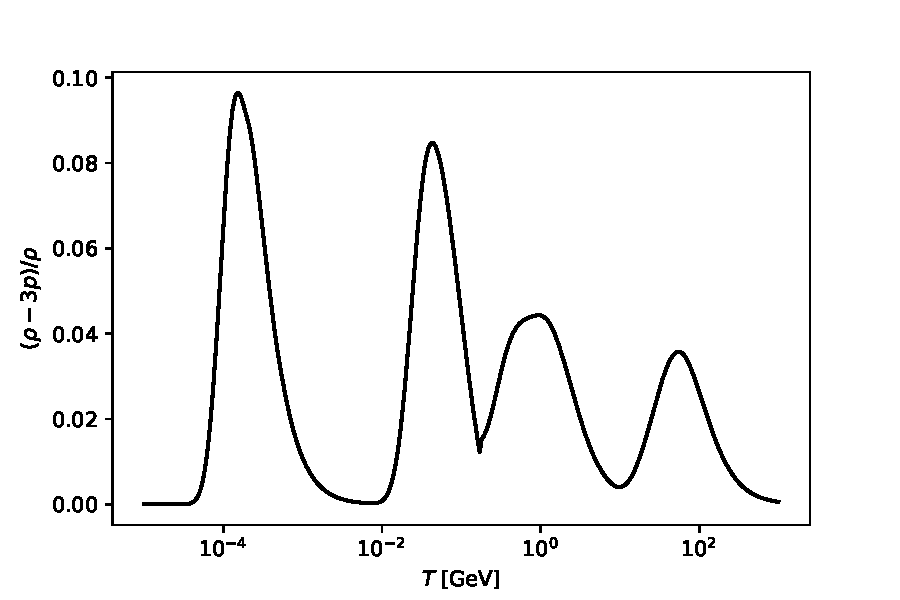
\includegraphics[scale=0.7]{figures/trace.pdf}% 图片在 Figures 文件夹中,注意修改尺寸大小 scale
\caption{能动量张量在宇宙早期随温度的演化。}% 图例
\label{trace}
\end{figure}

其中,
\begin{align}
    \rho-3 p=\frac{g T^{4}}{2 \pi^{2}} \cdot x^{2} \int_{0}^{\infty} d y \frac{y^{2}}{\sqrt{x^{2}+y^{2}}} \frac{1}{\exp\left(\sqrt{x^{2}+y^{2}}\right) \pm 1}
    \,. % 标点符号
    \notag % 不添加序号
\end{align}